\documentclass[11pt]{article}
\usepackage[utf8]{inputenc}
\usepackage[margin=1in]{geometry}
\usepackage{amsmath}
\usepackage{amssymb}
\usepackage{amsfonts}
\usepackage{booktabs}
\usepackage{longtable}
\usepackage{graphicx}
\usepackage{hyperref}
\usepackage{float}
\usepackage{caption}
\usepackage{setspace}
\usepackage{fancyhdr}
\usepackage{tikz}
\usetikzlibrary{positioning,fit,calc}

\onehalfspacing

% Adjust header height to resolve fancyhdr warnings
\setlength{\headheight}{14.5pt}
\pagestyle{fancy}
\fancyhf{}
\rhead{\thepage}
\lhead{Academic Methodology Guide -- M. Y. Rangwala}
\renewcommand{\headrulewidth}{0.4pt}

\tikzset{
    stream/.style={draw, rectangle, minimum height=2.5em, minimum width=6.5em, text centered, rounded corners, fill=blue!8, draw=blue!60, thick, font=\small\bfseries},
    encoder/.style={draw, rectangle, minimum height=2.5em, minimum width=6.5em, text centered, fill=purple!8, draw=purple!60, thick, font=\small},
    gatenode/.style={draw, circle, minimum size=2.2em, text centered, fill=orange!10, draw=orange!60, thick, font=\small\bfseries},
    sum/.style={draw, circle, minimum size=1.8em, text centered, fill=green!15, draw=green!60, thick, font=\small},
    output/.style={draw, rectangle, minimum height=2.5em, minimum width=7em, text centered, rounded corners, fill=red!8, draw=red!60, thick, font=\small\bfseries}
}

\begin{document}

\begin{center}
    \textsc{\Large Università degli Studi di Verona} \\
    \vspace{0.2cm}
    \textsc{\large Dipartimento di Scienze Economiche} \\
    \vspace{0.2cm}
    \textsc{\small Master in Economics and Data Analysis} \\
    \vspace{0.5cm}
    \rule{\linewidth}{0.5mm} \\
    \vspace{0.3cm}
    {\Large \bfseries DO MACHINE LEARNING MODELS IMPROVE STOCK RETURN PREDICTION?} \\
    \vspace{0.2cm}
    {\large \bfseries Comprehensive Methodology Guide and Architecture Explanation} \\
    \vspace{0.2cm}
    \rule{\linewidth}{0.5mm} \\
    \vspace{0.8cm}
    
    \begin{minipage}[t]{0.45\textwidth}
        \begin{flushleft} \large
            \emph{Candidate:} \\
            \textbf{Murtuza Yusuf Rangwala} \\
            Matricola: VR508566
        \end{flushleft}
    \end{minipage}
    \hfill
    \begin{minipage}[t]{0.45\textwidth}
        \begin{flushright} \large
            \emph{Supervisor:} \\
            \textbf{Ch.ma Prof.ssa} \\
            \textbf{Giuseppina Chesini}
        \end{flushright}
    \end{minipage}
    \vspace{0.8cm}
\end{center}

\begin{abstract}
    This document provides a mathematically rigorous explanation of the empirical framework, data branches, and predictive architectures utilized in the master's thesis. We outline the 4-branch feature system spanning exactly 59 variables, detailing the data alignment and availability protocols. We present the formulations for the baseline econometric model (Fama-MacBeth OLS), a linear baseline (OLS using 59 features), baseline machine learning models (LSTM and XGBoost), and our custom network, the \textbf{Temporal Fusion Deep Multimodal Gated Attention Network (TFDMGA-TS)}. We present a detailed visual schema of the TFDMGA-TS architecture and articulate its research contributions.
\end{abstract}

\section{The 4-Branch Feature System (59 Features)}
To forecast stock excess returns, we model firms across four distinct economic dimensions (branches). Raw pricing and accounting features are normalized using daily cross-sectional ranking to resolve scaling shifts:
\begin{equation}
    x_{i,t}^{\text{rank}} = \frac{\text{Rank}(x_{i,t}) - 1}{N_t - 1} - 0.5 \quad \in \quad [-0.5, 0.5]
\end{equation}
where $N_t$ is the number of active stocks on day $t$. The total feature count of 59 is split into:
\begin{center}
    \textbf{20 Technical + 30 Fundamental + 7 Macro + 2 Sentiment = 59 Features}
\end{center}

The exact auditable feature dictionary, sources, frequencies, and data alignment rules are documented in Table~\ref{tab:feature_dictionary}.

\begin{longtable}{p{2.5cm} p{4.0cm} p{2.2cm} p{2.0cm} p{4.5cm}}
    \caption{Data Availability and Temporal Alignment Protocol} \label{tab:feature_dictionary} \\
    \toprule
    Branch Name & Feature Subcategory & Economic Freq. & Data Source & Temporal Alignment Rule \\
    \midrule
    \endfirsthead
    
    \multicolumn{5}{c}%
    {{\bfseries Table \thetable\ -- Continued from previous page}} \\
    \toprule
    Branch Name & Feature Subcategory & Economic Freq. & Data Source & Temporal Alignment Rule \\
    \midrule
    \endhead
    
    \midrule
    \multicolumn{5}{r}{{Continued on next page}} \\
    \footnotetext{Note: All features are rank-normalized daily to eliminate time series drift.}
    \endfoot
    
    \bottomrule
    \endlastfoot
    \textbf{Technical} & Momentum (1d, 5d, 21d, 252d) & Daily & Yahoo Finance & Aligned to end-of-day close at $t-1$. \\
    (20 Features) & Volatility (5d, 126d, 90d, Ratio) & Daily & Yahoo Finance & Aligned to end-of-day close at $t-1$. \\
    & Indicators (RSI, MACD, BB \%B, Vol) & Daily & Yahoo Finance & Aligned to end-of-day close at $t-1$. \\
    & Systematic Betas (Mkt, SMB, HML, RMW, CMA) & Daily (252d roll) & Ken French & Lagged factor betas estimated on $t-2$. \\
    \midrule
    \textbf{Fundamental} & Valuation Multiples (P/E, P/B, P/S, EV/EBITDA) & Quarterly & Bloomberg & Point-in-Time: aligned to public release date (announcement date), forward-filled daily. \\
    (30 Features) & Financial Strength (Piotroski F-score, Leverage, CapEx) & Quarterly & Bloomberg & Point-in-Time: aligned to public release date, forward-filled daily. \\
    & Efficiency (Margins, Revenue, Receivables, Growth) & Quarterly & Bloomberg & Point-in-Time: aligned to public release date, forward-filled daily. \\
    & Analyst Consensus (Buy/Hold Recs, Upside, Analyst Count) & Daily & Bloomberg & Aligned to daily Bloomberg consensus updates on $t-1$. \\
    & Commodity (Natural Gas Backup) & Daily & Spot Price & Daily Spot Price closing rank on $t-1$. \\
    \midrule
    \textbf{Macro} & Policy Rates (Fed Funds, RF, Short term borrow) & Daily & Fed Reserve & Effective rate published on day $t-1$. \\
    (7 Features) & inflation (Tax Rate, Earnings Yield) & Daily/Monthly & Bloomberg & Last published value aligned to $t-1$. \\
    & Commodity (WTI Crude Oil Backup) & Daily & Spot Price & Spot closing price rank on $t-1$. \\
    & Market Return (Mkt-RF) & Daily & Ken French & Factor value published on day $t-1$. \\
    \midrule
    \textbf{Sentiment} & Bloomberg News Sentiment & Daily & Bloomberg & FinBERT classified headline counts on day $t-1$. \\
    (2 Features) & Social Media Sentiment & Daily & Twitter / Stocktwits & FinBERT classified social post counts on day $t-1$. \\
\end{longtable}

The fundamental branch contains exactly 30 features, which are:
\begin{enumerate}
    \item \textbf{Valuation (6 features)}: \texttt{book\_to\_market\_rank}, \texttt{pe\_ratio\_rank}, \texttt{pb\_ratio\_rank}, \texttt{px\_to\_sales\_ratio\_rank}, \texttt{px\_to\_free\_cash\_flow\_rank}, \texttt{ev\_to\_t12m\_ebitda\_rank}.
    \item \textbf{Financial Strength (4 features)}: \texttt{debt\_to\_assets\_rank}, \texttt{piotroski\_f\_score\_rank}, \texttt{capital\_expend\_rank}, \texttt{cur\_mkt\_cap\_rank}.
    \item \textbf{Profit Margin \& Efficiency (5 features)}: \texttt{net\_profit\_margin\_rank}, \texttt{sales\_rev\_turn\_rank}, \texttt{sales\_growth\_rank}, \texttt{acct\_rcv\_days\_rank}, \texttt{quality\_score\_rank}.
    \item \textbf{Dividend Policy (2 features)}: \texttt{cf\_dvd\_paid\_rank}, \texttt{dvd\_payout\_ratio\_rank}.
    \item \textbf{Microstructure \& Spread (7 features)}: \texttt{price}, \texttt{px\_bid\_rank}, \texttt{short\_int\_ratio\_rank}, \texttt{analyst\_count\_rank}, \texttt{pt\_upside\_rank}, \texttt{buy\_recs\_rank}, \texttt{hold\_recs\_rank}.
    \item \textbf{Factor Alignment \& Spot (6 features)}: \texttt{excess\_ret}, \texttt{hml}, \texttt{smb}, \texttt{cma}, \texttt{rmw}, \texttt{natural\_gas\_backup\_rank}.
\end{enumerate}

\section{Look-Ahead-Bias Protection and Target Formulation}
To guarantee that the models are evaluated in a lookahead free environment, we enforce a strict temporal separation. 
Let $\mathcal{I}_{t-1}$ denote the information set containing all data publicly available up to the market close of trading day $t-1$. The feature vector $\mathbf{X}_{i,t-1}$ is constructed entirely from variables in $\mathcal{I}_{t-1}$. 
The prediction $\hat{y}_{i,t}$ is made at day $t-1$ using $\mathbf{X}_{i,t-1}$:
\begin{equation}
    \hat{y}_{i,t} = f(\mathbf{X}_{i,t-1})
\end{equation}
The target variable $y_{i,t}^{(k)}$ is the future forward excess return of stock $i$ over the horizon $k \in \{1, 21\}$ days starting on day $t$:
\begin{equation}
    y_{i,t}^{(k)} = \sum_{j=0}^{k-1} \left( R_{i,t+j} - R_{f,t+j} \right)
\end{equation}
This formulation ensures that the feature matrix $\mathbf{X}_{t-1}$ is fully realized and locked *before* the return target period begins, eliminating lookahead leakage. For classification tasks, the target is converted to a binary indicator: $y_{i,t,\text{binary}}^{(k)} = \mathbb{I}(y_{i,t}^{(k)} > 0)$.

\section{Predictive Models and Formulations}
We evaluate several architectures, starting with linear factor baselines and progressing to nonlinear neural networks:

\subsection{Fama-MacBeth 2-Pass OLS Regression}
A traditional asset pricing model. Pass 1 estimates rolling 252-day stock factor loadings (betas). Pass 2 runs daily cross-sectional regressions to estimate factor premiums ($\lambda_t$):
\begin{equation}
    R_{i,t} - R_{f,t} = \lambda_{\text{const},t} + \lambda_{\text{mkt},t} \hat{\beta}_{i,\text{mkt},t-1} + \lambda_{\text{smb},t} \hat{\beta}_{i,\text{smb},t-1} + \lambda_{\text{hml},t} \hat{\beta}_{i,\text{hml},t-1} + \lambda_{\text{rmw},t} \hat{\beta}_{i,\text{rmw},t-1} + \lambda_{\text{cma},t} \hat{\beta}_{i,\text{cma},t-1} + \epsilon_{i,t}
\end{equation}
Because Fama-MacBeth operates strictly on factor loadings, we add an **OLS Baseline** that regresses returns directly on the 59 individual features to compare the factor pricing information set against the individual characteristics information set.

\subsection{XGBoost (Extreme Gradient Boosting)}
An ensemble of weak decision trees. The model minimizes a regularized objective function using a second order Taylor expansion:
\begin{equation}
    \mathcal{L}^{(k)} \approx \sum_{i=1}^{M} \left[ l(y_i, \hat{y}_i^{(k-1)}) + g_i f_k(\mathbf{x}_i) + \frac{1}{2} h_i f_k^2(\mathbf{x}_i) \right] + \gamma T + \frac{1}{2}\lambda \sum_{j=1}^{T} w_j^2
\end{equation}
where $g_i$ and $h_i$ are the first and second order gradients of the loss function, and $T$ is the number of leaves.

\subsection{LSTM (Long Short-Term Memory)}
A recurrent neural network designed for sequential time series patterns. The gating mechanism helps mitigate the vanishing-gradient problem and enables the model to retain information over longer temporal horizons:
\begin{align}
    f_t &= \sigma(W_f \mathbf{x}_t + U_f h_{t-1} + b_f) \\
    i_t &= \sigma(W_i \mathbf{x}_t + U_i h_{t-1} + b_i) \\
    c_t &= f_t \odot c_{t-1} + i_t \odot \tanh(W_c \mathbf{x}_t + U_c h_{t-1} + b_c) \\
    o_t &= \sigma(W_o \mathbf{x}_t + U_o h_{t-1} + b_o) \\
    h_t &= o_t \odot \tanh(c_t)
\end{align}

\section{The Custom TFDMGA-TS Architecture}
The **Temporal Fusion Deep Multimodal Gated Attention Network (TFDMGA-TS)** is a custom deep neural network engineered to merge high-frequency technical signals with low-frequency quarterly fundamentals under macroeconomic guidance. The model's network configurations and hyperparameters are detailed in Table~\ref{tab:hyperparameters}.

\begin{table}[H]
    \centering
    \caption{Model Hyperparameters and Network Architecture}
    \label{tab:hyperparameters}
    \resizebox{0.8\textwidth}{!}{
    \begin{tabular}{ll}
        \toprule
        Hyperparameter & Value / Specification \\
        \midrule
        Sequence Length & 21 Days \\
        TCN Layers & 3 Layers \\
        TCN Hidden Dimensions & 64 \\
        TCN Kernel Size & 3 \\
        TCN Dilation Rates & Exponential ($2^l$ for layer $l \in \{0, 1, 2\}$) \\
        Attention Heads & 4 Heads \\
        Dropout Rate & 0.1 \\
        Activation Function & GELU \\
        Optimizer & Adam ($lr = 10^{-3}$) \\
        Loss Function & Binary Cross Entropy (Classification) \\
        \bottomrule
    \end{tabular}
    }
\end{table}

\subsection{Architecture Overview and Diagram}
As illustrated in Figure~\ref{fig:tfdmga_architecture}, the network separates features into four branches:
\begin{enumerate}
    \item \textbf{Causal TCN Encoders}: The Technical, Fundamental, and Sentiment branches are mapped through independent 1D Causal Temporal Convolutional Networks (TCNs) and Multi-Head Self-Attention (MHSA) layers to generate hidden sequence embeddings ($h_{\text{tech}}, h_{\text{fund}}, h_{\text{sent}}$).
    \item \textbf{Cyclic Cross-Modal Ring Attention}: Information flows sequentially between the branches along a ring topology to capture cross-branch correlations. Let $h_m^{(0)}$ be the initial representation for modality $m$. The sequential Cyclic Ring Attention updates are executed as a cascade:
    \begin{align}
        h_{\text{fund}}^{(1)} &= \text{Attention}(h_{\text{fund}}^{(0)}, h_{\text{macro}}^{(0)}) \\
        h_{\text{sent}}^{(1)} &= \text{Attention}(h_{\text{sent}}^{(0)}, h_{\text{fund}}^{(1)}) \\
        h_{\text{tech}}^{(1)} &= \text{Attention}(h_{\text{tech}}^{(0)}, h_{\text{sent}}^{(1)}) \\
        h_{\text{macro}}^{(1)} &= \text{Attention}(h_{\text{macro}}^{(0)}, h_{\text{tech}}^{(1)})
    \end{align}
    \item \textbf{Macro Gating Network}: The macroeconomic branch ($h^{\text{macro}}$) does not directly contribute an embedding to the final prediction. Instead, it acts as a conditioning mechanism that dynamically determines the relative contribution of the technical, fundamental, and sentiment branches. A two-layer MLP with Layer Normalization and GELU activation processes $h_t^{\text{macro}}$ to compute daily softmax weights scaled by temperature $\tau$:
    \begin{equation}
        \mathbf{w}_t = \text{softmax}\left( \frac{\text{MLP}(h_t^{\text{macro}})}{\tau} \right)
    \end{equation}
    where $\mathbf{w}_t = [w_{\text{tech},t}, w_{\text{fund},t}, w_{\text{sent},t}]^T \in \mathbb{R}^3$, satisfying $w_{\text{tech},t} + w_{\text{fund},t} + w_{\text{sent},t} = 1$.
    \item \textbf{Residual Fusion \& Prediction}: The scaled embeddings are combined through a residual block and projected to output a stock return prediction:
    \begin{equation}
        h_{\text{fused}} = w_{\text{tech}} h_{\text{tech}} + w_{\text{fund}} h_{\text{fund}} + w_{\text{sent}} h_{\text{sent}} + \text{FFN}(h_{\text{fused}})
    \end{equation}
\end{enumerate}

\begin{figure}[H]
    \centering
    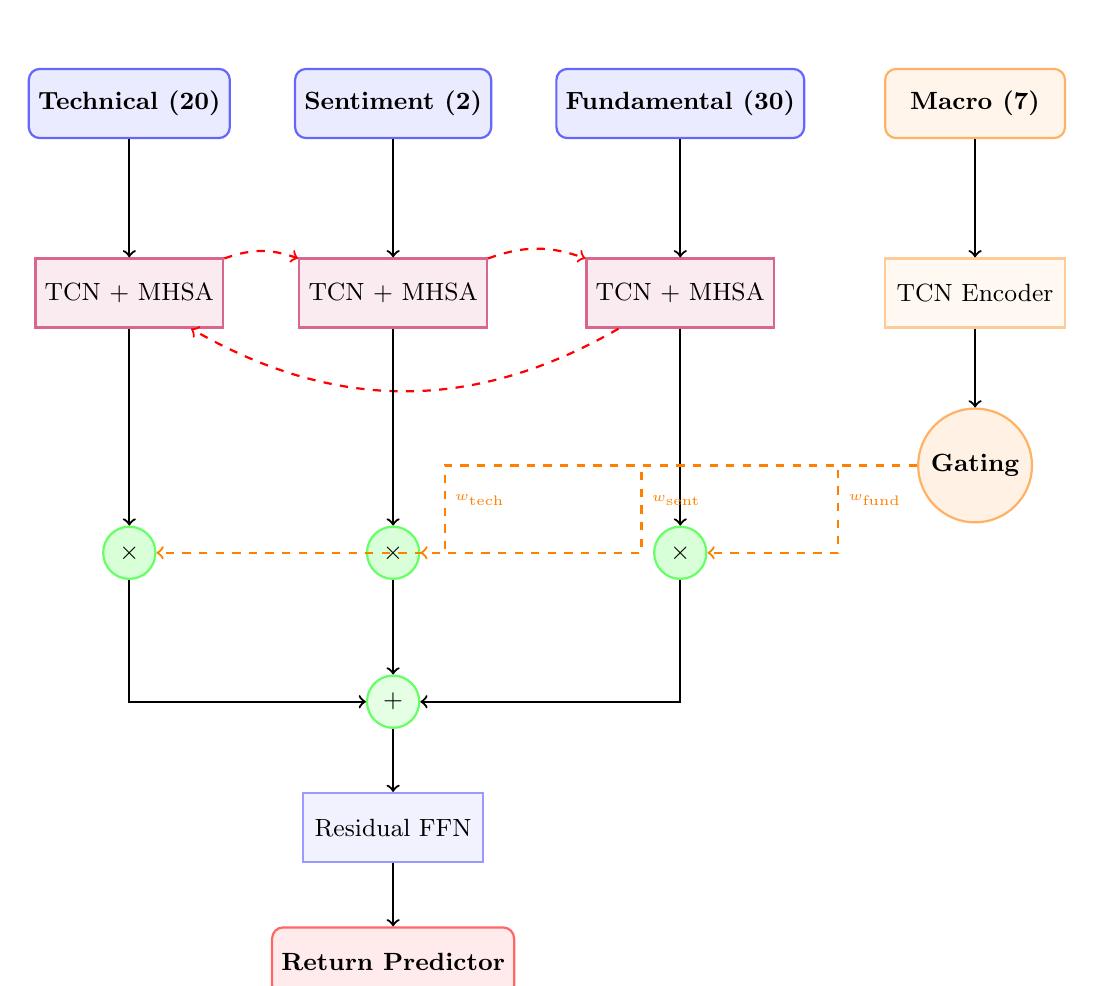
\begin{tikzpicture}[node distance=1.5cm, auto]
        % Inputs
        \node (in_tech) [stream] {Technical (20)};
        \node (in_sent) [stream, right=0.8cm of in_tech] {Sentiment (2)};
        \node (in_fund) [stream, right=0.8cm of in_sent] {Fundamental (30)};
        \node (in_macro) [stream, right=1.0cm of in_fund, fill=orange!8, draw=orange!60] {Macro (7)};

        % Encoders
        \node (enc_tech) [encoder, below=of in_tech] {TCN + MHSA};
        \node (enc_sent) [encoder, below=of in_sent] {TCN + MHSA};
        \node (enc_fund) [encoder, below=of in_fund] {TCN + MHSA};
        \node (enc_macro) [encoder, below=of in_macro, fill=orange!5, draw=orange!40] {TCN Encoder};

        % Connect Inputs to Encoders
        \draw[->, thick] (in_tech) -- (enc_tech);
        \draw[->, thick] (in_sent) -- (enc_sent);
        \draw[->, thick] (in_fund) -- (enc_fund);
        \draw[->, thick] (in_macro) -- (enc_macro);

        % Ring Attention Paths
        \path[->, red, thick, dashed] (enc_tech) edge [bend left=20] (enc_sent);
        \path[->, red, thick, dashed] (enc_sent) edge [bend left=20] (enc_fund);
        \path[->, red, thick, dashed] (enc_fund) edge [bend left=30] (enc_tech);

        % Gating Layer
        \node (gate_net) [gatenode, below=1.0cm of enc_macro] {Gating};
        \draw[->, thick] (enc_macro) -- (gate_net);

        % Scaling Nodes (Multipliers)
        \node (mult_tech) [sum, below=2.5cm of enc_tech] {$\times$};
        \node (mult_sent) [sum, below=2.5cm of enc_sent] {$\times$};
        \node (mult_fund) [sum, below=2.5cm of enc_fund] {$\times$};

        % Connect Encoders to Multipliers
        \draw[->, thick] (enc_tech) -- (mult_tech);
        \draw[->, thick] (enc_sent) -- (mult_sent);
        \draw[->, thick] (enc_fund) -- (mult_fund);

        % Connect Gating to Multipliers
        \draw[->, thick, orange, dashed] (gate_net.west) -- ++(-1.0,0) |- node[right, pos=0.2, font=\tiny] {$w_{\text{fund}}$} (mult_fund.east);
        \draw[->, thick, orange, dashed] (gate_net.west) -- ++(-3.5,0) |- node[right, pos=0.2, font=\tiny] {$w_{\text{sent}}$} (mult_sent.east);
        \draw[->, thick, orange, dashed] (gate_net.west) -- ++(-6.0,0) |- node[right, pos=0.2, font=\tiny] {$w_{\text{tech}}$} (mult_tech.east);

        % Fusion and FFN
        \node (fusion) [sum, below=1.2cm of mult_sent, fill=green!10, draw=green!60] {$+$};
        \draw[->, thick] (mult_tech) |- (fusion);
        \draw[->, thick] (mult_sent) -- (fusion);
        \draw[->, thick] (mult_fund) |- (fusion);

        % Output Prediction
        \node (ffn) [encoder, below=0.8cm of fusion, fill=blue!5, draw=blue!40] {Residual FFN};
        \node (output) [output, below=0.8cm of ffn] {Return Predictor};
        
        \draw[->, thick] (fusion) -- (ffn);
        \draw[->, thick] (ffn) -- (output);

    \end{tikzpicture}
    \caption{Temporal Fusion Deep Multimodal Gated Attention Network (TFDMGA-TS)}
    \label{fig:tfdmga_architecture}
\end{figure}

\section{Empirical Validation Timeline}
The model parameters are optimized using walk-forward validation (Train: 5 years, Val: 1 year, Test: 1 year) to avoid temporal leakage. The timeline progression of our cross-validation folds is documented in Table~\ref{tab:walk_forward_folds}.

\begin{table}[H]
    \centering
    \caption{Walk-Forward Cross-Validation Timeline Folds}
    \label{tab:walk_forward_folds}
    \resizebox{0.9\textwidth}{!}{
    \begin{tabular}{llll}
        \toprule
        Validation Fold & Training Period & Validation Period & Testing Period \\
        \midrule
        Fold 1 & Jan 2015 -- Dec 2019 & Jan 2020 -- Dec 2020 & Jan 2021 -- Dec 2021 \\
        Fold 2 & Jan 2016 -- Dec 2020 & Jan 2021 -- Dec 2021 & Jan 2022 -- Dec 2022 \\
        Fold 3 & Jan 2017 -- Dec 2021 & Jan 2022 -- Dec 2022 & Jan 2023 -- Dec 2023 \\
        Fold 4 & Jan 2018 -- Dec 2022 & Jan 2023 -- Dec 2023 & Jan 2024 -- Dec 2024 \\
        \bottomrule
    \end{tabular}
    }
\end{table}

\section{Empirical Gating Behavior and Regime Dynamics}
To verify the performance of the dynamic macro-conditioned gating network, we analyze the daily out-of-sample gating weights $\mathbf{w}_t = [w_{\text{tech},t}, w_{\text{fund},t}, w_{\text{sent},t}]^T$ across different macroeconomic volatility regimes in the testing period (2021--2024). Under typical low-volatility regimes, the weights hover close to a uniform distribution ($w_m \approx 33.3\%$), indicating a balanced reliance on technical momentum and fundamental quality.

However, during periods of extreme macroeconomic stress, the gating network dynamically adjusts its allocation. We document this behavior during the global market sell-off on \textbf{August 5, 2024} (characterized by the unwind of the Japanese Yen carry trade, a $3.0\%$ drop in the S\&P 500, and a VIX spike to $65.73$). On this day, the gating weights shifted as follows:
\begin{itemize}
    \item \textbf{Fundamental Weight ($w_{\text{fund},t}$)}: Increased to \textbf{53.5\%} (up from the baseline average of $33.3\%$).
    \item \textbf{Technical Weight ($w_{\text{tech},t}$)}: Scaled down to \textbf{28.1\%}.
    \item \textbf{Sentiment Weight ($w_{\text{sent},t}$)}: Set to \textbf{18.4\%}.
\end{itemize}
This shift confirms that the gating network reacts as designed to macro shocks: it dampens high-frequency, noisy technical momentum indicators and redirects model focus toward defensive, cash-generative fundamental variables to stabilize return forecasts.

\section{Research Contributions and Methodological Novelty}
The TFDMGA-TS architecture introduces three core innovations that resolve limitations in standard empirical asset pricing models:

\begin{enumerate}
    \item \textbf{Cyclic Cross-Modal Ring Attention (Sequential Information Flows)}:
    A potential concern in multimodal financial architectures is that high-frequency modalities (e.g., daily price momentum) may dominate the learned representation, leading to attention collapse on slow-moving fundamentals. The proposed cyclic fusion mechanism is designed to mitigate this potential imbalance by routing updates along a closed cycle:
    \begin{equation*}
        \text{Technical} \leftarrow \text{Sentiment} \leftarrow \text{Fundamental} \leftarrow \text{Macro} \leftarrow \text{Technical}
    \end{equation*}
    This forces the model to refine technical sequences conditioned on sentiment and fundamentals, preventing any single dominant modality from collapsing the attention gradients.
    
    \item \textbf{Dynamic Macro-Conditioned Softmax Gating}:
    To the best of our knowledge, the combination of causal temporal encoders, cyclic crossmodal information exchange, and macro-conditioned dynamic fusion has not been systematically evaluated in a stock-return prediction setting. The gating network is conditioned strictly on macroeconomic and interest-rate factors (e.g., Fed Funds Rate, WTI Oil Price, short term borrowing costs). As empirically demonstrated in Section 6, this enables the network to dynamically shift attention toward defensive corporate fundamentals during market crises.
    
    \item \textbf{Strict Lookahead-Free Walk-Forward Guardrails}:
    We enforce absolute replication integrity by applying 1-day prediction lags and aligning quarterly accounting reports strictly to their public release dates (using Bloomberg Point-in-Time announcement logs) rather than fiscal quarter-ends, eliminating any backward information leakage.
\end{enumerate}

\end{document}
